\part{Análise e Desenvolvimento de Sistemas}\label{ParteII}

\chapter[Análise e Desenvolvimento de Sistemas]{Análise e Desenvolvimento de Sistemas}\label{Capitulo3}

\section{Visão Geral}

Desenvolvimento de sistemas baseia-se essencilamente, em seguir umas série de etapas.
Sistemas de informação são importantes para as organizações porque podem melhorar seu desempenho e representar um diferencial competitivo, logo isso agrega mais valor ao negócio da organização~\cite{alvarenga2016efeitos}.

A demanda do mercado de Tecnologia da Informação (T.I.) é impulsionada pela importância que os sistemas de informação representam para as organizações.
Neste cenário, os provedores de soluções em T.I. devem atender a determinados critérios, tais como desenvolver exatamente o que foi demandado, cumprir o cronograma planejado e manter os custos estejam próximos do que foi estimado inicialmente~\cite{alvarenga2016efeitos}.

\section{Metodologias de Desenvolvimento de Software}

As metodologias tradicionais de desenvolvimento de software, tem a característica de documentação extensiva, e pela ordem e disciplina no decorrer do desenvolvimento, garantindo um controle rígido dos processos~\cite{baltzan2016tecnologia}.

Um tipo de metodologia tradicional é o modelo cascata que tem como principal característica a divisão do projeto em etapas que seguem uma sequência linear, onde a próxima se inicia somente após o término da anterior e essas metodologias tradicionais são consideradas rígidas e burocráticas~\cite{baltzan2016tecnologia}.

Com isso as metodologias ágeis são adotadas como uma opção às abordagens tradicionais de desenvolvimento de software por ter como foco ciclos de vida adaptativos, os quais são reativos a altos níveis de mudança e envolvimento contínuo das partes interessadas~\cite{vargas2014manual}.

Metodologias ágeis utilizam, portanto, um processo iterativo e incremental, e são adaptativas às mudanças que podem ocorrer, exigindo o mínimo de documentação possível, com foco total no desenvolvimento de código~\cite{vargas2014manual}.

Scrum é uma metodologia ágil utilizada para gestão e planejamento de software.
É indicado para equipes pequenas e tem o foco principal de garantir uma forma de trabalho flexível em ambientes onde a mudança é constante, isto é, requisitos, recursos, tecnologia e outras variáveis técnicas podem se tornar obstáculos complexos no ambiente do projeto~\cite{dos2004metodologias}.
O Scrum é adequado a ambientes com muitas mudanças por sua flexibilidade frente aos desafios que surgem em tais ambientes~\cite{dos2004metodologias}.

Logo, a adoção do Scrum como metodologia de gerenciamento do projeto, se dá pelo fato de ser mais vantajosa para uma equipe pequena que busca agilidade.
E além disso, o Scrum é uma das mais populares metodologias no mercado atualmente, conforme mostrado na~\prototipo{Figura001}~\cite{paulk2013scrum}.

\begin{figure}[htbp]
    \centering
    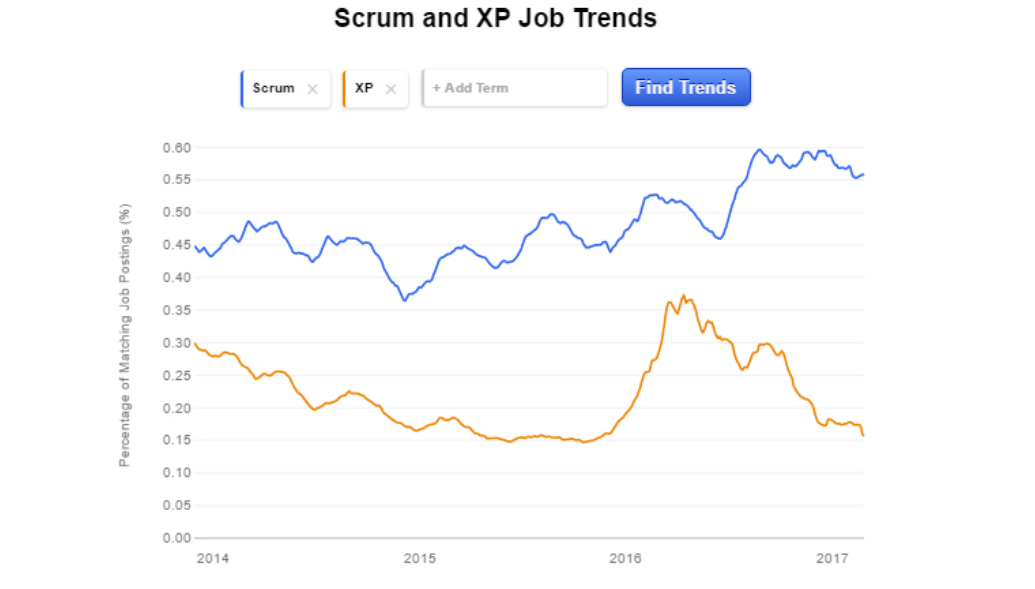
\includegraphics[width=0.95\textwidth]{figuras/figura001.png}
    \caption[Figura 1: Demanda por profissionais de Scrum e XP]{Demanda por profissionais de Scrum e XP, duas metodologias ágeis de gerenciamento de projetos, entre 2014 e 2017~\cite{mazuco2017percepccoes}.}
    \label{Figura001}
\end{figure}.

\section{Levantamento de Requisitos}

Vários estudiosos da indústria de software, durante a década de 70, caracterizaram os problemas relacionados ao desenvolvimento de software como uma ``crise'', então o levantamento de requisitos tem como principal motivação a especificação, desenvolvimento e manutenção de sistemas~\cite{sommerville2007engenharia}.

Por meio do uso de modelos abstratos e precisos, o levantamento de requisitos permite modelar um sistema, de modo que todos os passos do desenvolvimento de um software atinjam um resultado esperado e atendam às expectativas do cliente~\cite{pressman2016engenharia}.

Desta forma o levantamento de requisitos é ao mesmo tempo uma necessidade do projeto e um risco.
Se os requisitos forem por algum motivo alterados, o investimento em levantá-los terá sido perdido~\cite{schimiguel2017tecnicas}.

Nas metodologias tradicionais, para se manter um requisito conciso ao final do levantamento, os requisitos são avaliados e em seguida é criado um escopo junto ao cliente para que ele se comprometa a não adicionar novas funcionalidades no período de execução do projeto~\cite{lutz2018implantaccao}.
Em metodologias ágeis a gerência de requisitos é mais flexível.


Para descrever os requisitos podem ser usado os casos de uso, que são narrativas em texto que servem como registro de requisitos do sistema para atingir as metas esperadas pelo o usuário.
Os casos de uso servem como um conjunto de cenários relacionados que identificam o fluxo da informação, detalhando como será o caminho do usuário para atingir o objetivo~\cite{larman2002utilizando}.

\section{Implementação}

Implementação é a fase posterior ao levantamento de requisitos.
Que consiste nas atividades de desenvolver os componentes do sistema através de programação, e desenvolver o banco de dados através do modelo de dados~\cite{azevedo2008definiccao}.
%Disso, geralmente resulta a configuração de como vai ser feito, quais pacotes de software usar e como deverá ser acessado.

\subsection{Aplicação web}

Uma aplicação web é qualquer software que é executado em um navegador.
Elas são mantidas e atualizadas sem a necessidade de distribuir e instalar software em computadores dos clientes, diferente das aplicações tradicionais que dependem dessa necessidade~\cite{sampaio2004xwebprocess}.

O desenvolvimento de uma aplicações web é geralmente feito por equipes multidisciplinares, com diferentes habilidades.
Há diversas vantagens frente aos sistemas convencionais, como o acesso em qualquer plataforma mobile ou computador pessoal, integração com outros sistemas e um \textit{front-end} amigável enquanto o \textit{back-end} pode ser complexo~\cite{ferreira2015arquitetutura}. 

\subsubsection{\textit{Back-end}}

O \textit{back-end} da aplicação é a parte responsável por armazenar e processar e prover dados para que as aplicações possam usar de diversas maneiras.
O \textit{back-end} é onde os dados do sistema são processados e armazenados.
É onde se encontra toda a parte de regras de um sistema~\cite{silva2017aplicaccao}.

\subsubsection{\textit{Front-end}}

O \textit{front-end} corresponde à interface encontrada ao acessar um aplicação, na intranet ou na web.
Nela é possível encontrar a parte de navegação, inserção de informação ou consulta, por isso o \textit{front-end} é toda a parte da aplicação que interage diretamente com o usuário~\cite{de2016estudo}.

\subsubsection{\textit{Framework}}

Os \textit{frameworks} são esqueletos de uma aplicação e possuem conjuntos já definidos e diversas estruturas prontas que são códigos comuns entre vários projetos de software.
\textit{Frameworks} provêem de forma genérica algumas funcionalidades que pode ser melhoradas e tornadas mais específicas durante a implementação~\cite{minetto2007frameworks}.

O benefício do uso de \textit{frameworks} durante a implementação é o aumento da agilidade no processo de implementação, gerando redução de custos e suporte a resolução de problemas~\cite{nash2003java}.

\subsubsection{REST}
 \textit{Representational State Transfer} (REST) é uma arquitetura baseado no protocolo \textit{HyperText Transfer Protocol} (HTTP) que serve para definir como é a comunicação entre sistemas de informação e a transferência de dados entre eles.
Essa arquitetura usa o conceito de cliente-servidor, no qual são obtidos recursos através de \textit{endpoints} utilizando os métodos HTTP~\cite{pacheco2018institutos}.

\subsection{Ferramentas}

% Para a implementação de uma aplicação web precisamos saber quais ferramentas que serão utilizadas.

\subsubsection{Linguagem de Programação}

As linguagens de programação são utilizadas como meio de comunicação entre computadores e desenvolvedores. 
Elas permitem que especifiquemos quais ações podemos tomar para situações diferentes~\cite{costa2017colossus}.

Uma linguagem de programação é um procedimento padronizado que expressa as instruções através de conjunto de regras sintáticas e semânticas para definir um programa de computador.
As regras sintáticas fazem referência a forma de escrita, às regras semânticas e ao conteúdo~\cite{gotardo2015linguagem}.

Em desenvolvimento web existem dois tipos de linguagens de programação as \textit{client-side} que fica no \textit{front-end} e as \textit{server-side} que fica na parte do \textit{back-end}.

As linguagens \textit{client-side} são responsáveis pelas ações executadas no cliente, nesse caso no navegador.
Essas linguagens têm com função a validação de dados e o dinamismo de apresentação de dados.
Além da linguagem de programação, a linguagem de marcação estrutura de como vai ser a página, enquanto os \textit{scripts} de estilização definem a aparência do \textit{front-end}~\cite{silveira2015desenvolvimento}.

As linguagens \textit{server-side} são responsáveis pelas ações executadas no servidor web.
A linguagem de programação nesse caso irá interpretar os dados e retornará dados para ser exibidos no navegador, tendo como principal uso, as consultas e regras do sistema~\cite{campos2007realidade}.

\subsubsection{Banco de Dados}

Um sistema de banco de dados é um sistema computadorizado de manutenção de registros cuja finalidade é armazenar informações e permitir que o usuário busque e atualize essas informações quando solicitado~\cite{date2004introduccao}.

%Então banco de dados pode ser definido como uma coleção organizada de dados e esses dados são armazenados e estruturados de forma a permitir agilidade na busca e na recuperação por um computador~\cite{manovich2015banco}.

%Nessa parte do banco de dados existe uma ferramenta para auxiliar o gerenciamento de dados.

O Sistema gerenciador de banco de dados é responsável pelo gerenciamento de um banco de dados, e retira do do usuário a responsabilidade de gerenciar diretamente o acesso, a manipulação e a organização dos dados.
O usuário interage através de uma interface com os dados armazenados através de uma linguagem que é usada para fazer consulta chamada \textit{Structured Query Language} (SQL)~\cite{laundon2007sistemas}.

\subsubsection{API}

 \textit{Application Programming Interface} (API) é um conjunto estabelecido de mensagem que utilizam os métodos HTTP, que irão enviar resposta ou trazer mensagem e essas troca de informação geralmente é feito com o \textit{Javascript Object Notation} (JSON) ou \textit{eXtensible Markup Language} (XML).
 As duas têm a mesma aplicação o que muda são apenas as estruturas de troca de mensagem em relação a apresentação e a escolha delas será feita pela tecnologia que tem disponibilidade para utilizar ou não~\cite{oliveira2015desenvolvimento}.

\subsection{Tecnologias}

%Sabendo quais ferramentas serão utilizadas para a implementação de uma aplicação web precisamos de definir quais tecnologias que serão utilizadas no back-end e front-end.

\subsubsection{Java}

Java$^{\tiny{\textregistered}}$ é uma linguagem de programação que pode ser utilizada para programar sistemas computacionais em alto nível~\cite{batista2017desenvolvendo}. 
Vários sistemas de transações, chats, games e aplicações web são construídos em Java.

\subsubsection{Spring boot}

O\textit{ Spring boot} é um \textit{framework} que acelera a programação de aplicações Java$^{\tiny{\textregistered}}$ simplificando e abstraindo complexidades de configuração, muitas vezes repetitivas~\cite{bianchi2015sistema}.

\subsubsection{JPA e Hibernate}

O \textit{Hibernate} permite a comunicação entre a aplicação e o banco de dados através de \textit{Java Persistence API} (JPA).
JPA permite à aplicação salvar, ler, atualizar e excluir e consultar dados do banco de dados~\cite{gonccalves2007desenvolvendo}.

\subsubsection{MySQL}

O MySQL é um Sistema Gerenciador de Bancos de Dados (SGBD) aderente a \textit{Atomicity, Consistency, Isolation and Durability} (ACID), compatível com operações \textit{Create, Read, Update, Delete} (CRUD), que combina flexibilidade de esquema com integridade de dados~\cite{mysql2018}.


\subsubsection{HTML}

O \textit{Hypertext Markup Language} (HTML) é uma linguagem de marcação que serve para estruturar a apresentação e conteúdo de uma aplicação web através de etiquetas que são chamadas de \textit{tags}~\cite{agustin2015model}.

\subsubsection{CSS}

A estilização do HTML pode ser feita através de \textit{Cascading Style Sheets} (CSS), as quais definem em atributos, a aparência de componentos do \textit{Document Object Model} \textit{DOM}, como tamanho da fonte ou cores, por exemplo~\cite{abreu2016desenvolvimento}.

\subsubsection{JavaScript}

JavaScript é uma linguagem de programação web.
Uma de suas principais funcionalidades é fornecer interatividade nas aplicações originalmente estáticas~\cite{de2016estudo}.

\subsubsection{Bootstrap}

O \textit{Bootstrap} é um \textit{framework} que é utilizado para a padronização de interface da aplicação, ele é composto por componentes HTML, CSS, e JavaScript, gerando assim um desenvolvimento ágil e permitindo que as páginas sejam adaptáveis aos mais variados dispositivos que as acessam~\cite{pereira2017ferramenta}. 

\subsubsection{AngularJS}

O AngularJS é um \textit{framework} JavaScript que pode ser usado para o desenvolvimento de aplicações web e mobile.
É baseado em um modelo que centraliza a aplicação em uma única página executada através do navegador.
Ele busca os dados do servidor sem a necessidade de atualização completa da página.
Sua estrutura ajuda na comunicação com o \textit{back-end} e com as rotas das páginas~\cite{de2016estudo}.

Hackerrank\footnote{https://www.hackerrank.com} e StackOverflow\ref{https://stackoverflow.com/} são dois portais de Internet largamente utilizados pela comunidade de desenvolvedores. E por isso, dispôem de informação sobre o uso de tecnologias ao redor do mundo.
Em~\prototipo{Figura002},~\prototipo{Figura003}, e~\prototipo{Figura004} podemos ver dados estatísticos retirrado destes portais.
Esses dados reforçam a relevância das tecnologias escolhidas para o desenvolvimento do produto alvo deste trabalho.


\begin{figure}[htp]
    \centering
    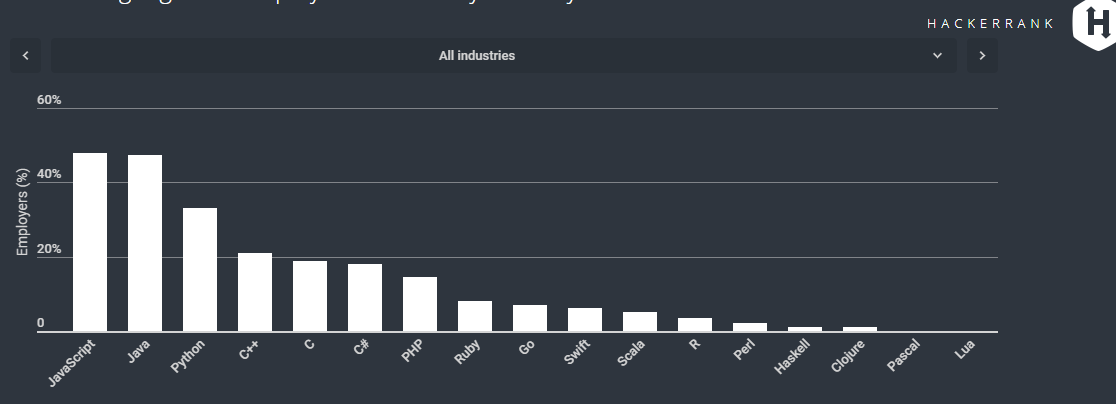
\includegraphics[width=0.95\textwidth]{figuras/figura002.png}
    \caption{Linguagens de programação mais demandadas pela indústria de software~\cite{linguagemEframework}.}
    \label{Figura002}
\end{figure}

\begin{figure}[htp]
    \centering
    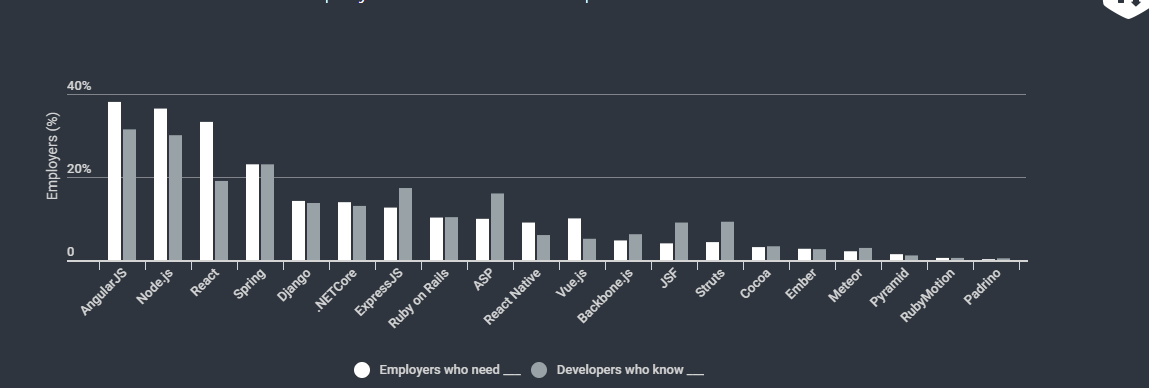
\includegraphics[width=0.95\textwidth]{figuras/figura003.png}
    \caption{Comparativo entre frameworks demandados e nível de conhecimento dos mesmos pelos desenvolvedores~\cite{linguagemEframework}.}
    \label{Figura003}
\end{figure}

\begin{figure}[htp]
    \centering
    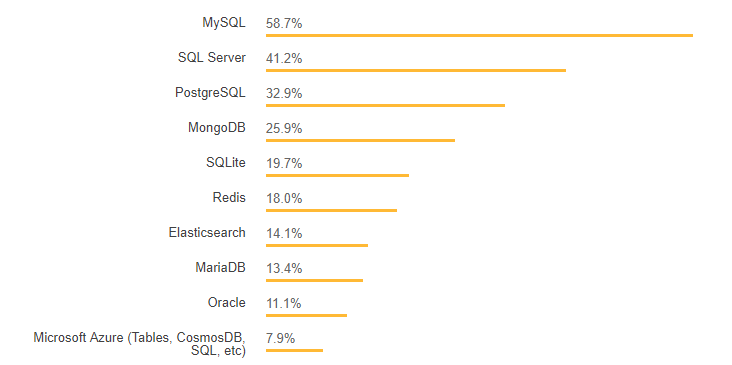
\includegraphics[width=0.95\textwidth]{figuras/figura004.png}
    \caption{Bancos de dados mais usados no mundo em 2017 segundo o portal StackOverflow~\cite{bancomaisusado}.}
    \label{Figura004}
\end{figure}

\section{Homologação e Implantação}

A homologação é a fase onde o cliente e os interessados pelo produto, verificaram que o software feito atende aos critérios de aceite previamente estabelecidos com o cliente. 
Essa atividade inicia-se após correção dos erros encontrados em testes feitos pelos clientes e interessados, caso em que a homologação é considerada finalizada com sucesso~\cite{santos2017cp}.

A implantação ocorre apenas depois da homologação.
Após a aprovação do cliente o produto é entregue, e o cliente pode implantar o software em seu ambiente de produção~\cite{pressman2016engenharia}.
Na produção podem aparecer problemas ainda não detectados.
Caso haja impacto nas atividades, sejam eles falhas de definições de requisitos, desenvolvimento divergente às regras definidas ou erros no código, volta-se ao ciclo de desenvolvimento para aprimorar as funcionalidades que tem problemas~\cite{salvador2015processo}.

Para controlar as versões, o produto obedece a um modelo chamado versionamento semântico.
Versionamento semântico é uma proposta simples de regras e requisitos que ditam como os números das versões são atribuídos e incrementados~\cite{palestino2015estudo}. 
Exemplo de formato de versão: $X.Y.Z$ (Maior.Menor.Correção).

\begin{itemize}
    \item X(Maior): quando ocorrem mudanças incompatíveis.
    \item Y(Menor): quando são adicionadas funcionalidades mantendo compatibilidade.  
    \item Z(Correção):  quando são corrigidas as falhas mantendo compatibilidade. 
    
\end{itemize}

Quando um software é lançado recebe a o número de versão $1.0.0$.
O \textit{maior} (X) geralmente é usado para uma nova versão de software que recebera grandes modificações.
Quando o software recebe melhorias o \textit{menor} (Y) é adicionado $1.1.0$ e quando recebe correções é adicionado o \textit{correção} (Z) correção $1.1.1$~\cite{versionamento}.


\section{Processo de Software}

Processo de software é um conjunto de atividades e resultados associados que produzem um produto de software~\cite{sommerville2007engenharia}.
Essas atividades são inter-relacionadas ou interativas.
Dentre as atividades mais importantes podemos destacar:

\begin{itemize}
	\item Especificação de software: define as pricipais funcionalidades do software e suas restrições.
	\item Design e implmentação do software: define como osoftware deve ser desenhado e programado.
	\item Verificação e validação: define a conformidadade entre a necessidade do usuário e a especificação do software.
	\item Manutenção do software: define modificações alinhadas à mudanças de requisitos.
\end{itemize}

%Optamos por uma metodologia ágil, que é mais indicada para cenários como o nosso, equipe pequena e prazo curtos.
%Com ela pudemos aplicar um fluxo de forma mais ágil, levantamos os requisitos, identificamos os problemas e definimos as soluções.
%Em seguida, documentamos essas soluções através dos casos de uso e iniciamos a implementação, adotando as tecnologias e arquitetura com as quais temos mais experiência.
%Mantivemos o fluxo ágil na fase de homologação e esperamos atingir o que o cliente espera.

